\documentclass[10pt]{beamer}
\usetheme{metropolis} % Modern theme, requires 'metropolis' package
\usepackage{bookmark}
\usepackage{tikz}
\usetikzlibrary{shapes.geometric, arrows}
\usepackage{booktabs}
\usepackage{pgfgantt}

% Colors
\definecolor{primary}{HTML}{10b981} % Teal
\definecolor{secondary}{HTML}{0f172a} % Deep Navy
\setbeamercolor{palette primary}{bg=secondary, fg=white}
\setbeamercolor{title}{fg=primary}

\title{Unio: Unified Marketplace \& Trust Platform}
\subtitle{Collective Buying and Community Verification System}
\author{Team Members: [Member 1] ([ID]), [Member 2] ([ID]) \\ Guide: [Name of Guide]}
\date{\today}
\institute{[University Name]}

\begin{document}

\maketitle

% Slide 2
\begin{frame}{Introduction}
    \begin{itemize}
        \item \textbf{Unio} is a multi-dimensional platform bridging commerce and community.
        \item Combines specialized logistics (Cargo/Storage) with a feature-rich marketplace.
        \item Core innovation: A \alert{Decentralized Trust Layer} that weights peer P2P interactions.
    \end{itemize}
\end{frame}

% Slide 3
\begin{frame}{Problem Statement}
    \begin{itemize}
        \item \textbf{Fragmentation}: Users jump between apps for logistics, buying, and community chat.
        \item \textbf{Trust Gap}: High cognitive load for verifying sellers or service providers in P2P sharing.
        \item \alert{Inefficiency}: Expensive luxury items remain inaccessible without cooperative buying models.
    \end{itemize}
\end{frame}

% Slide 4
\begin{frame}{Project Objectives}
    \begin{enumerate}
        \item Build a unified ecosystem for diverse P2P services.
        \item Implement a \textbf{Co-Purchase Split} engine for high-value items.
        \item Develop a data-driven \textbf{Trust Score} algorithm based on verified shared experiences.
    \end{enumerate}
\end{frame}

% Slide 5
\begin{frame}{Purpose and Need}
    \begin{itemize}
        \item \textbf{Cost Optimization}: Sharing the burden of high-cost assets (e.g., specialized gear).
        \item \textbf{Security}: Reducing fraud through a verified community rating system.
        \item \textbf{User Experience}: Single-login access to logistics, auctions, and social groups.
    \end{itemize}
\end{frame}

% Slide 6
\begin{frame}{Scope of the Project}
    \begin{columns}
        \column{0.5\textwidth}
        \textbf{Marketplace}
        \begin{itemize}
            \item Real-time Auctions
            \item Fixed-price Listings
            \item Split Purchases
        \end{itemize}
        \column{0.5\textwidth}
        \textbf{Community}
        \begin{itemize}
            \item Trust Scoring (P2P)
            \item Friends/Social Circle
            \item Real-time Chat
        \end{itemize}
    \end{columns}
\end{frame}

% Slide 7
\begin{frame}{Social Relevance \& SDGs}
    \begin{itemize}
        \item \textbf{SDG 12: Responsible Consumption}: Unio promotes the "Sharing Economy," reducing waste.
        \item \textbf{SDG 11: Sustainable Communities}: Strengthening local ties through collaborative buying.
        \item \textbf{Social Impact}: Democratizing access to expensive equipment through co-ownership.
    \end{itemize}
\end{frame}

% Slide 8.1
\begin{frame}{Functional Requirements}
    \begin{itemize}
        \item \textbf{Authentication}: Secure JWT-based login/signup.
        \item \textbf{Listing Management}: Multi-category support (Vehicles, Electronics, etc.).
        \item \textbf{Transaction Engine}: Bidding history and Split-payment state management.
        \item \textbf{Social Engine}: Friend requests and verified peer reviews.
    \end{itemize}
\end{frame}

% Slide 8.2
\begin{frame}{Non-functional Requirements}
    \begin{itemize}
        \item \textbf{Scalability}: Modular Node.js routes for easy feature extension.
        \item \textbf{Responsiveness}: Fluid UI using Tailwind CSS grid/flex layout.
        \item \textbf{Security}: Encrypted password storage via Bcrypt; SQL injection prevention.
    \end{itemize}
\end{frame}

% Slide 9
\begin{frame}{System Architecture}
    \centering
    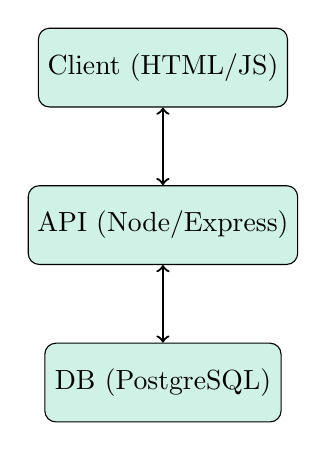
\begin{tikzpicture}[node distance=2cm]
        \tikzstyle{box} = [rectangle, rounded corners, minimum width=3cm, minimum height=1cm,text centered, draw=black, fill=primary!20]
        \node (client) [box] {Client (HTML/JS)};
        \node (api) [box, below of=client] {API (Node/Express)};
        \node (db) [box, below of=api] {DB (PostgreSQL)};
        \draw [thick, <->] (client) -- (api);
        \draw [thick, <->] (api) -- (db);
    \end{tikzpicture}
\end{frame}

% Slide 10
\begin{frame}{Application Architecture Design}
    \begin{itemize}
        \item \textbf{Backend Layout}: 
            \begin{itemize}
                \item \texttt{server.js}: Entry point \& Middleware.
                \item \texttt{routes/}: Discrete logic for \texttt{splits}, \texttt{trust}, \texttt{marketplace}.
            \end{itemize}
        \item \textbf{Database Persistence}: \texttt{db.js} handles connection pooling and automated schema initialization.
    \end{itemize}
\end{frame}

% Slide 11
\begin{frame}{GUI Design (Mockups)}
    \begin{itemize}
        \item \textbf{Theme}: Deep Navy (#0f172a) based Glassmorphism.
        \item \textbf{Interactions}: 
            \begin{itemize}
                \item Sliding activity drawer for notifications and chats.
                \item Centered modals for split creation and bidding.
            \end{itemize}
    \end{itemize}
\end{frame}

% Slide 12
\begin{frame}{API Design}
    \footnotesize
    \begin{tabular}{llp{4cm}}
    \toprule
    \textbf{Endpoint} & \textbf{Method} & \textbf{Purpose} \\
    \midrule
    \texttt{/api/splits/create} & POST & Initialize co-purchase \\
    \texttt{/api/marketplace/bids} & POST & Submit auction bid \\
    \texttt{/api/trust/rate} & POST & Verified peer rating \\
    \texttt{/api/auth/login} & POST & Secure session setup \\
    \bottomrule
    \end{tabular}
\end{frame}

% Slide 13
\begin{frame}{Database Design}
    \begin{itemize}
        \item \textbf{Total Tables}: 15+ Relational Tables.
        \item \textbf{Key Schema}: 
            \begin{itemize}
                \item \texttt{users} $\rightarrow$ \texttt{listings} $\rightarrow$ \texttt{bookings}
                \item \texttt{marketplace\_items} $\rightarrow$ \texttt{split\_requests} $\rightarrow$ \texttt{split\_members}
            \end{itemize}
        \item \textbf{Optimization}: Indexes on \texttt{user\_id} and \texttt{item\_id} for faster joins.
    \end{itemize}
\end{frame}

% Slide 14
\begin{frame}{Technology Stack}
    \begin{itemize}
        \item \textbf{Language}: JavaScript (ES6+).
        \item \textbf{Framework}: Express.js (v5.0 alpha support).
        \item \textbf{Database}: PostgreSQL (v16+).
        \item \textbf{Styling}: Tailwind CSS (CDN/Utility-first).
        \item \textbf{Runtime}: Node.js with PM2 process monitoring.
    \end{itemize}
\end{frame}

% Slides 15-19: Modules
\begin{frame}{Module: Marketplace \& Auctions}
    \begin{itemize}
        \item \textbf{Auction Engine}: Automated countdowns and highest-bidder locking.
        \item \textbf{Listing Flow}: Seller dashboard for item creation with image uploads.
        \item \textbf{Real-time Sync}: Periodic polling to update bid statuses without page refresh.
    \end{itemize}
\end{frame}

\begin{frame}{Module: Marketplace Splits}
    \begin{itemize}
        \item \textbf{Philosophy}: Collaborative buying to reduce individual financial burden.
        \item \textbf{Flow}: Creator sets slots $\rightarrow$ Member joins with terms $\rightarrow$ Group confirms purchase.
        \item \textbf{Calculation}: Proportional price splitting per slot.
    \end{itemize}
\end{frame}

% Slides 20-25: Algorithms
\begin{frame}{Algorithm 1: Auction Concurrency}
    \begin{enumerate}
        \item Fetch Current Bid $\rightarrow$ Validate New Bid $>$ Current + Increment.
        \item Start DB Transaction.
        \item Update \texttt{highest\_bidder\_id} and \texttt{current\_bid}.
        \item Commit Transaction $\rightarrow$ Notify outbid users.
    \end{enumerate}
\end{frame}

\begin{frame}{Algorithm 2: Trust score calculation}
    \begin{equation}
        Score(U) = \frac{\sum_{i=1}^{n} (Rating_i)}{n} \times Weight(Experience)
    \end{equation}
    \begin{itemize}
        \item Experience Weight: Verified shared booking $>$ Friend rating $>$ Public rating.
    \end{itemize}
\end{frame}

% Slide 26: Environment
\begin{frame}{Coding Standards \& Environment}
    \begin{itemize}
        \item \textbf{Version Control}: Git (Branching for features/bugfixes).
        \item \textbf{Environment}: Dotenvx for secure secret management (\texttt{.env}).
        \item \textbf{Standards}: camelCase for JS, snake\_case for DB columns.
    \end{itemize}
\end{frame}

% Slides 27-30: Testing
\begin{frame}{Testing Methodology}
    \begin{itemize}
        \item \textbf{Unit}: Validation of bid amounts and split price divisibility.
        \item \textbf{Integration}: Verification of JWT token persistence across routes.
        \item \textbf{Load}: PM2 clustering tests to handle concurrent API requests.
    \end{itemize}
\end{frame}

% Slide 31: Bug Report
\begin{frame}{Bug Management}
    \begin{itemize}
        \item \textbf{Resolved}: 404 Route errors due to zombie node processes.
        \item \textbf{Resolved}: Front-end loading hang caused by stale DOM references.
        \item \textbf{Optimization}: Periodic inbox polling improved chat responsiveness.
    \end{itemize}
\end{frame}

% Slide 38: Conclusion
\begin{frame}{Conclusion}
    \begin{itemize}
        \item \textbf{Unio} provides a viable blueprint for trust-based P2P platforms.
        \item Successfully integrated logistics, marketplace, and social verification.
        \item Future work: Blockchain-based payment escrow and AI-driven fraud detection.
    \end{itemize}
\end{frame}

% Slide 39: Bibliography
\begin{frame}{Bibliography}
    \begin{itemize}
        \item [1] ExpressJS.com - Official Documentation.
        \item [2] PostgreSQL.org - Database Manual.
        \item [3] TailwindCSS.com - Styling Reference.
        \item [4] Node.js Foundation - Best Practices.
    \end{itemize}
\end{frame}

\end{document}
